\newpage
\section{Process Environment}


% Kill di un processo in C
\subsection{Kill di un processo in C}

Per far \hl{terminare un processo} usiamo:

\begin{enumerate}
    \item \hl{return} dal main
    \item chiamando \hl{exit}: \textbf{chiudo la singola thread} ma poi passa da un \textbf{gestore di exit (exit function)} che chiama gli \txtbf{exit handler} che possono essere installati e aggiunti tramite la funzione
\begin{lstlisting}
int atexit(void (*func)(void));
\end{lstlisting}
    e verranno richiamate in ordine contrario alla dichiarazione
    
    \item chiamando \hl{\_exit o \_Exit}: usate per terminare il processo e \textbf{finire direttamente nel kernel} senza passare dall'exit function
    \item \hl{return dell'ultima thread}
    \item chiando \hl{pthread\_exit dall'ultima thread}
    \item chiamando \hl{abort}: che \textbf{genera un segnale gestibile SIGABRT}, ma che fa comunque teminare il processo
    \item ricevendo un \hl{segnale}: come \textbf{SIGKILL e SIGSTOP} che non potranno essere gestiti o fermati
    \item \hl{richiesta di cancellazione} dell'ultima thread
\end{enumerate}


% Environment list
\subsection{Environment list}

Quando si va a \hl{creare una variabile} nello schell:

\begin{lstlisting}
$ a=100
\end{lstlisting}

questa \hl{non viene passara al child schell}, come "env", a meno di non \hl{usare il builtin "export"}.

In un processo \hl{possiamo vedere le variabli di ambiente in runtime}, tramite il debugger, ma non nello stesso punto in cui si trovano. \hl{Per le variabili di ambiente} abbiamo che:


\begin{figure}[H]
\centering
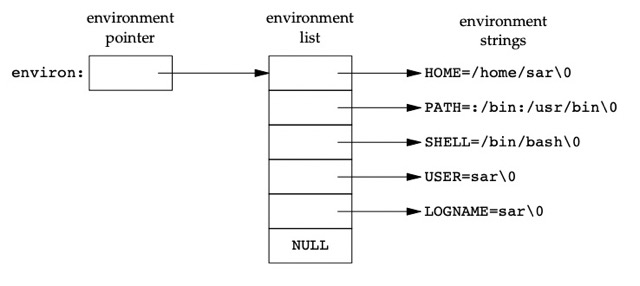
\includegraphics[scale=0.4]{varamb.jpeg}
\caption{Variabili di ambiente} 
\label{varamb}
\end{figure}


dove ogni valore è \hl{separato da un null $\backslash 0$} e \hl{storicizzato in un array di puntatori} andando a terminare con un null.

I programmi, tramite un \hl{handle}, possono \hl{accedere a questo array tramite un altro puntatore} (environment pointer), come:

\begin{lstlisting}
extern char **environ;
\end{lstlisting}

oppure nel \hl{main}:
\begin{lstlisting}
int main(int argc, char *argv[], char *envp[]);
\end{lstlisting}

oppure con la \hl{funzione}:
\begin{lstlisting}
char *getenv(const char *name);
\end{lstlisting}

che \hl{passando il nome della variaible di ambiente restituendo un puntatore al suo contenuto}.

Notare che la \hl{malloc usa zone globali allora non è rientrant}, vedremo poi cosa vuol dire.






(VEDERE memory\_dump.c) che vede e sampa tutte le variabili di mabinete, aspetta un p`o e poi lo ri fa stampandone anche di nuove e modificandone una esistente e poi va a vedere rispetto ai punttori precendenti c se sno ancora buoni  o se stanno da un altra parte

vedere a mush simpler way to print addresses used in process memory per stampare semplicemtne gli indirizzi delle variabili di ambiente


in memory\_dump.c abbiamo un popen che restituisce un puntatore di tipo file che e1 uin ingresso alla pipe [in pratica ]

con sort -n ordine numerico -r reverce -k3 chiave (colonna) da scegliere con w dico che la triga la vogli scrivere nella pipe

notiamo che le libreire di namiche stanno da tutaltra parte delle funzioni che osno del programma che sono come puntatori al text (stano in basso)
infatti vediamo con $(()) che abbimao 216 byte tra i puntato di envp0 e envp27 con $(()) notiamo che abbiamo solo 64 bit a sisposizione id cui uno e1 per il segno in quel caso usiamo bc

il programma vuole capire cosa succedere alle variabilei di imabiente quando vanno modificate o agiunte

putenv: mette direttamente dove sono le variabili di ambiente prende una tringa cheha tutta la variabile di ambiente: name=value e se c'e1 gia1 non fa nulla
setenv: si appoggia di una memoria alllocata

negli if crea delle variabili con putenv e vuole andare a vedre dove sono

display var ambient:
loop sulle variabili di ambiente e setta "\&" poi in strncopy copia un buf+1 la stringa della varaibile prendendo size buf-2 perche togliamo $\backslash 0$ e \&
per printare fa un mkPrintable per evitare di avere strani segni nell'output
dumpAddr() fa una fprintf nel puntatore per dargli la riga da sptampre



una pipe e1 una struttura con ...

dato che popen onn e1 sicura faccio la chiamata pipe una fork e poi il chil una exec del sort


strchr: isola in nome della variaible e poi nell'if vede se il nome e1 TERM, se TERM e1 definita e verifca se il puntatore vero e1 diverso da quello nuovo e quindi vede se la variabil e1 stat cambiata
allora aggancia a TERM @ e = e poi aggiunge l'ltimo agiornamtne della varaibile di ambiente (quella cambiata) 
con cp che indica dove e1 stata spostata la varaibile

qindi le nuove varaibili modificate sanno inun tunto della memoria diverso da quello iniziale dato che in genre son incastarete tra loro tramite un unica stringa ma separate da un \0 allora si e1 pensato di carearne direttamente un altra in un altro punto di memoria e la get env si preoccupa di fare tutto e di dire che non si deve piu fare affidamente al vecchio puntatore alla variabile ma al nuovo

ricordare che 
gli standard fanno rispettare le interfaccie e non le implementazioni quindi fanno rispettare parametri e return della funzione ma non cosa fa dentro

per vedere le aree di memoria per le quali il porcesso ha il permesso:
vmmap -resident ointerleaved 9163

su linux 
cat /proc/$$/maps


setjump e longjump:

serve quando hai tanti stack frame che hanno fatto elaborazioni lunghe e lo stack siallunga, allora nell'ultima chiamata potremmo volr uscre e rifare il corcorso al contratrio per chiuderela tendina degli stack frame allora quando dienta lunga puo esser comodo dire di togliere tutti li stack frame e andare direttametn allinizio. fiunziona con le chiamate setjump e longjump
1. la fa nella funzione chiamante nela qule si vuole fare il return per esmpio di puo ritorna alla prima, eliminando tutti le azioni intermedie perche no nci soddisfa un valore e vlgiamo rincomunicare da zero. allora si passa al setjump una fotografica del tipo della variabile jmp\_buf env. questa prima chiamata fa return di zero per dirti che la foto della varaibiel sta storizzata bene. se poi volgiamo ritornare allinizion tramite longjumop si ritorna setjump passandogli la fotografi jmp\_buf env e anceh un int val che rappresenta, come se avessi fatto la setjump solo che gil fa ritornare la variabile val impostando il valore del return della setjump. dato che puoessere chiamata da tanti posti al longjump allora ritorna un numero diverso in base a dove si trovano


ad ogni processo si posson ogestire is uoi limiti: come con setrlimit e gerlimit

si basa tutto su una struttura fatta da un campo con illimite corrente ed uno con li limite massimok (hard limit)

struct rlimit{
...
}

la chiamata è fatta da: 

RLIMIT_NPROC
RLIMIT_CPU


soft limit: il prcesso funziona e podo n min non può piu andare

int getrlimit(...)

setrlimit: gli passi una struttra che è stata già riempita e poi gli dai i limiti da iporre:
1. il porcesso puo cambaire un soft limit sotto all'hard limit puoi fare tutto so[ra no


hard limit: il porcesso non puo duperarlo mai come limite 

2. un porocesso puo autolimitarsi abbassando l'hard limit corrente, questo abbassamento è irreversibile per un utente normal
3. solo il superuser puo cambiare l'hardlimit

l'hard limit di un tuo porcessoi lo puo cambiare come ti pare
un porcesso puo fare o no qualcosa tramite i limiti, user normale puo cambiare i soft, il superuser puo cambiare l'hard


in base ai constanti possiamo trovare i limite per piu misurazioni (?)
sono delle costanti dato che vanno a restituire un valore intero che raffigura il limite

fig7.16

il programma inizia con una particolarità sta nella macro dato he è una funztion like ma c'è un #name dove viene passato il nome della costante e poi in name il suo valore

vediamo che RLIM_INFINITY è dati da ((_uint64)1 << 63) - 1)

RLIMIT_CORE: limite current che se 0 vuol dire che al momento del crash del sistema le immagini non vengono salvate 

per vedere i limiti correnti uso:

$ ulimit -a
core file size          (blocks, -c) 0
data seg size           (kbytes, -d) unlimited
file size               (blocks, -f) unlimited
max locked memory       (kbytes, -l) unlimited
max memory size         (kbytes, -m) unlimited
open files                      (-n) 2560
pipe size            (512 bytes, -p) 1
stack size              (kbytes, -s) 8176
cpu time               (seconds, -t) unlimited
max user processes              (-u) 2666
virtual memory          (kbytes, -v) unlimited


questo, se lanciati in bash sono i limiti di bash









cap 8: process control

nonostante abbiamo un parent ed un child avremoche i file desriptor del child puntano agli stessi del parent sullo status flag (che possiamo cambiare tramite i un'opzione di fcntl
abbiamo ainfatti che intern process communications ara necessaria dato che se qualcosa la sciver ilhild se la rtrova il parent

besides the open files, numerous other properties of the parent are inherited by the child:
- real user id, real group id, effective user id, effective group id
- terminale di controllo: terminale colquale sta dialogando il porcesso i deamon non ne hanno
- root direcorty: dove sta la root
- fil emode creation mask: umask
- memory mappings
- resource limits

differenza tra parent e child
- file locks per mettere daccordo 2 file su un blocco di memoria da usare


funzione wait
	undo un poiircesso fa un child il parent vuole sapre cosa stia facendo il chidld, allor ail sistemama mantine delle info per capire cosa fa es: se sta continuando o è stato killato ad un cero punto il child conclude e chiude allora il kernel non butta via le infodato che le deve dare al parent aspetando che lo interroghi

questo stato viene detto lo stato dei porcessi zombie dato che il prcesso child è morto ed il parent non vuole saperne nulla, allora le info rimangono li ma senza che mai interrogate, per questo zombie

se il nostro procesos parent è uscito ed ha chiuso allo rarimuove l'info zombie 

per evitare di fare la wait si fa una dobbia fork chiudendo il proc di mezzo reclamendo prima la info dal secondo.

un altra tecnica per risolvere il problema della wait è di non fare wait & subito. usiamo il segnale SIGCHILD che viene mandato al proceso quando un child ha terminato, allora mettiamo al wai t all'arrvi di equesto segnali, infatti la wait non chiede u pid del porcesso che stai a septtando termini allora potra cosi termianre per un qualsiasi child termini 

sai come è andato a finire tutto in 
pid_t wait(int *statloc);
waitpid puo esser bloccante 
pid_t waitpid(pid_t pid, int *statloc, int options);


se abbiamo che è il parent a chiudere prima del child, allora il parent diventa il processi 1 che per definizione non ha wait quindi le info andreanno perse

 per capire da quale segnale il porocesso è stato fermato EIFSTOPPED(status)

 WIFSIGNALED(status) dice ceh segnaele `e stato inviato al processo

 wai t puo essere fatta inq ualsiasi processo il chiamante puo daprer che il child e1 stato stoppato e non chiuso e quindi poter usare uina tlra wait per poter aspettare che le info arrivino


 es:
 fig8.6

 la wait fa il return del pid del child (correggere sopra)

 pr_exit mettere code1


 se vogliamo aspettare la temrinazione di uno specifico processo

 watipid jha delle opzioni: la poiu importante WNOHANG (non rimane appenso ad aspettare)il return è 0 sara o oinvocaara tramite sifchild o ogni tanto si vede se ha temrinato, WCONTINUED se si supporta il job control per poter conrollare l'esegiuimento del processo, fermarlo, metterlo in background.


fig8.8 chiamo una doppia fork





race conditions:
situioni dove il risultato di una elaborazione cambia in base a chi arriva prima in maniera imprevedibile edindesiderata

fig8.12

permette di veder il race condition in azione ma con lepresatzioni dei pc di ora non funzione quidni usare suna sleep o meglio una usleep

per evitare le race condiioniton ci vengono in cotnro le sincoronizzazioni dato che vogliamo che siano sincronizzati tra loro i porcessi
i modi sono tantissimi, nel nostro esempi ousiamo delle unfioni in apue.h tramite dei segnali 


il sistema fa ad ogni porceso u ntime slice cio che quel porcesso riesce a fare in quel time slice 

come soluzioni possiamo vedere:
TELLWAIT() inizializza la faccenda


tellwait2

va tutto bene






exec functions:

execl (list): sequenza di argomentiseparati da una "," e castati con 0 , paso i parametri trami telista
int execl(cost char *pathname, const char *arg0, ... /* (char *) */;

terminatore lista (char *)0
allora possiamo avere che pathname e1 il path del programmae in arg0 mettiamo il nome del porgramma che potrebbe anceh essere un altro ed in queto caso alcuni programmi possono fare cose diverse in base al nome

execlp (path): passo il path del filename
int execlp(

execv (vector): passiamko gli argomenti come vettore
char *vector[] = {..,...,}
...

exece (environment): varaibili di ambiente pasare tramite vettore
...


se si fa una exec il pid cambia del porcesso. vengono ereditate:

- value ...
- close-onoexec flag che indica se il file descriptor deve essere chiuso o meno 


fig8.16

con flag 0 andiamo ad aspettare che l'altro child finista (waitpid)
env_int[] per sceglieere quale e1 l'ambiente ceh vogliamo usare, in alternativa lo eredita. ha un NULL finale per dire che e1 finito il vettore

terzo if eredito l'ambinte



guardare perche non si mette il punto nel path

per evitare questa cosa scriviamo 

$ PAH=. ./exec1

in modo da passargli . come path senza incorrere in porblemi di sicurezza


guarda echoall.c




chenge userID:
si vuole cambiare identia quando si e1 eseguito un orogramacon set uaser id attivo, vuoi uscire dalla root. alcuni programmi con pswd danno i privileggi e settano il set user id bit solo mentre fanno quell'alzione e poi la rilasciano per farti ritornare ad essere un normal user. i nuovi sistemi ofrono un timbro che ti permette di avere un saved set user id per poter permettere delle porzioni di programma senza essere super user e poi diventarlo solo quando serve. rappresenta un migliormeto di sicurezza dal settare sempre i lset user id bit.



interpreter files:
si riferisce ai programmi che iniziano con
#! pathname[ptional-argument]

es: #!/bin/sh

serve per poter eseguire il file in un certo modo come se facessimo sh [filename]





system function:
la "system" call delega le operazioni del programma a dei programmi esterni (pericolosa dato che i file pure se vengono cambiati saranno eseguiti
system()





valore di nice: permette di abbassare la priorita1 piu e1 alta piu sei carino (nice) men opirorita hai quindi si incemnte il numero per aumentarla si usa un -1

setpriority
getpriority






process times:
lo otteniamo di sonolito in bashcon la keyword "time"

real	0m0.000s
user	0m0.000s
sys	0m0.000s

lo usiamok ora come porgramatori che ti da i tempo dei porcesso e la puoi fare qundo ti pare durante il programma per monitorare l'evolzione del programma. si lavora con i ticks cioe una suddivisione dei sevondi che pero non e1 un valore fissato ma dipende dalla macchina (in genere e1 100) sarebbero i clock ticks

CLOCKTICKSPERSECOND = 100
sysconf(SC_CLK_TCK)

clock_t times(struct tms *buf)

un budf vengon omessi i risultati

struct tms {
	...
}

il valore di ritorno da il tempo reale passato

times1.c


getrusage: (esempi su moodlis)
int getrusage(int who, struct rusage *r_usage);

timeval = microsecondi

struct rusage {
             struct timeval ru_utime; /* user time used */
             struct timeval ru_stime; /* system time used */
             long ru_maxrss;          /* max resident set size */
             long ru_ixrss;           /* integral shared text memory size */
             long ru_idrss;           /* integral unshared data size */
             long ru_isrss;           /* integral unshared stack size */
             long ru_minflt;          /* page reclaims */
	     long ru_majflt;          /* page (4k byte) faults (dice se delle pagine sono state mappate dato che non è nella memoria fisica)*/
             long ru_nswap;           /* swaps */
             long ru_inblock;         /* block input operations */
             long ru_oublock;         /* block output operations */
             long ru_msgsnd;          /* messages sent */
             long ru_msgrcv;          /* messages received */
             long ru_nsignals;        /* signals received */
             long ru_nvcsw;           /* voluntary context switches */
             long ru_nivcsw;          /* involuntary context switches */
};

ma non restituisce il valore di clock reale

il tempo viene dato in microsecondi per avere quello reale usiamo gettimeofday


vedere come funziona il programma




























inseriamo la nuova cartella e vediamo il numero di eseguibili: find . -type f -perm -0100

compiliamo il make file ignorando gli errori: make -i 

crea il file di compilazione .sh
-D_XOPNE_SOURCE=600 forzata da fuori fa rispettare il susv3


per leggere i core file che osno una foto del porcesso della sua meroira e dei registri nel moento in cui il porcesso riceve un segnale. il rilascio del core non e1 garantito dato che c'e1 ilproblema del core file size

lo vediamo cin ulimit -a che ce lo dice a proporito di un processo ovviamnente che lo fara ereditare ai suoi child.
per cambiarlo e farlo unlimited:
ulimit -c unlimited

il che e1 molto pericoloso dato che crea moltissime "foto"

bash prima che arrivi il sengale al child fa una wait, fa la foto e poi continua. i fleg sono WIFSIGNALED e poi per sapere se ha rilasciato il core usa WCOREDUMP
il core viene messo in:


su mac usiamo "sysctl -a" che tira fuori molti parametri alcuni scrivibili solo da amministratore 
il aprametro che ci interessa e1 kern,coredump

$ sysctl -a | grep core
kern.corefile: /cores/core.%P
kern.coredump: 1
kern.sugid_coredump: 0
machdep.cpu.cores_per_package: 8
machdep.cpu.core_count: 8



guardando il file producecore.c vediamo che fallisce dato che il puntatore int *p = 0 e1 assegnato ad una variabile id memoria non accessibili cioe 0

questo con core file size = 0

se la modifichiamo il programma andra1 

il file creato avra lo stickybit attivo


guardare file how to examine ...

per linux gdb producecore core.1234

pe rmacos lldb producecore e poi diamok il numero di core

con info reg o register read possiamo vedere su linux e mac i registri nel memtno i ncui e1 successo il pasticcio cioe1 e1 arrivato il segnale









VEDERE SYSTEM CALL 
su linux:

eseguire un prgramma e vedere tutte le system call che il porgramma fa:
strace -t -v

dove t trappresenta la raffinatezza per quanto rigurada il tempo
dove v fa il verbose di tutti dati e non gli tronca
